\section{Introduction}
	\begin{wrapfigure}{r}{0.3\textwidth}
		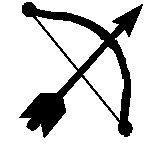
\includegraphics[width=0.3\textwidth]{../Images/c6/BOVIL.jpg}
		\label{fig:bovil}
	\end{wrapfigure}

	% % TODO 666 intro de la web
	The code and the documentation of the library can be found in the website \cite{BOViL}
	
\section{Content}
	The library is divided in to main sections:
	\begin{itemize}
		\item \textit{Core}: This section include some basics that could be helpful in every kind of application and algorithm; as an easy socket implementation, matrix operations, timing, and so on.
		\item \textit{Algorithms}: In this section are implemented a variety of algorithm; as the color clustering used and described in this project and the EKF tracking algorithm for ground and flying targets.
	\end{itemize}
	
	\subsubsection{Core}
		\begin{itemize}
			\item \textit{Communication}: Fast implementation of cross-platform sockets. The use is described on the wiki and accept any kind of UDP and TCP/IP sockets.
			\item \textit{Math}:
				\begin{itemize}
					\item \textit{Matrix}: \textit{Easy to use} matrix implementation.
					\item \textit{Geometrics}: Linear subspace class implementation.
				\end{itemize}
			\item \textit{Time}: Cross-platform time management.
			\item \textit{Types}: Basic types used in the library
		\end{itemize}
		
	\subsubsection{Algorithms}
		\begin{itemize}
			\item \textit{Segmentation}: Implementation of segmentation algorithm. At present, only color-based segmentation is implemented.
			\item \textit{State Estimators}: 
			\begin{itemize}
				\item \textit{ExtendedKalmanFilter}: Basic template of Extended Kalman Filter. It's used to implement easily any kind of EKF overriding the jacobians.
				\item \textit{GroundEKF}: derived class of \textit{ExtendedKalmanFilter} that override its jacobian for ground tracking.
				\item \textit{StereoEKF}: derived class of \textit{ExtendedKalmanFilter} that override its jacobian for stereo tracking.
			\end{itemize}
		\end{itemize}